\documentclass[b5paper,fleqn]{ltjsarticle}
\usepackage{amsmath,amsfonts,tikz}\usetikzlibrary{automata}\tikzset{initial text=}
\newcommand\s[1]{\subsection*{#1}\noindent\ignorespaces}
\newcommand\sbs[1]{\subsubsection*{#1}}
\newcommand\al[1]{\begin{align*}#1\end{align*}}
\newcommand\tx{\intertext}
\newcommand\ex[1]{\vskip5pt\underline{\bf 例}\quad#1\par}
\renewcommand{\labelenumi}{\alph{enumi}).}
\title{オートマトンと言語}
\author{大阪分散技術コミュニティ}
\begin{document}
\maketitle

\begin{description}
\item [タイトル] オートマトンと言語
\item [著者] Michael Sipser
\item [訳者] 太田和夫,田中圭介
\item [出版日] 2008/5/21
\item [出版社] 共立出版
\item [ISBN10] 4320122070
\item [ISBN13] 978-4320122079
\item [ページ数] 240
\item [言語] ja
\item [内容]MIT屈指の名講義の講義ノートをまとめた書
\end{description}

\section{Notation}
使用する記号と用語についてまとめる。
\begin{description}
\item[$\Sigma$: Alphabet] 空でない有限集合
\item[$s$: Symbol(文字)] アルファベットの元
\item[$\omega$: String over an alphabet] 有限の文字列
\item[$|\omega|$: Length] 文字列の長さ
\item[$\varepsilon$: Empty string(空列)]$|\varepsilon|:=0$
\item[$L$: Language(言語)] 文字列の集合
\item[$\Sigma_\varepsilon:=\Sigma\cup\{\varepsilon\}$]
\item[$2^A$:] Aのべき集合 
\item[$\mathbb{N}$:] 0を含む自然数
\end{description}
$w=s_1s_2\cdots s_n$であり、文字列と文字は区別される。$|w|=n$である。
\s{star(スター演算)}
集合$A$に対してスター演算を以下で定義する。
\[A^*=\{x_1x_2\cdots x_k|x_i\in A,k\in\mathbb{N}\}\]
\ex{$\Sigma=\{0,1\}$とすると、$\Sigma^*=\{\varepsilon,0,1,00,01,10,11,\cdots\}$
}
\section{Automaton}
Finite Automaton(有限オートマトン)を以下で定義する。
\[M=<Q,\Sigma,\delta,q_0,F>\]
\begin{description}
\item[$Q$: States(状態集合)] 空でない有限集合
\item[$\Sigma$: Alphabet] 空でない有限集合
\item[$\delta$: Transition functions(遷移関数)] $Q\times\Sigma\rightarrow Q$
\item[$q_0$: Start state(開始状態)] $q_0\in Q$
\item[$F$: Set of accept states(受理状態集合)] $F\subset Q$
\end{description}
\section{State Diagram}
状態遷移図
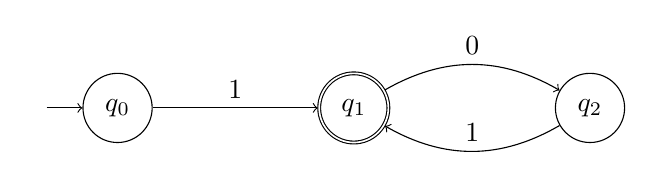
\begin{tikzpicture}[node distance=3cm]
\node[state,initial](q0){$q_0$};
\node[state,accepting,right of=q0](q1){$q_1$};
\node[state,right of=q1](q2){$q_2$};
\draw[->](q0)--node[above]{$1$}(q1); 
\draw[->,bend left](q1)edge node[above]{$0$}(q2)(q2)edge node [above] {$1$}(q1); 

\end{tikzpicture}

\section{Nondeterministic Automaton}
先述の定義はDeterministic Finite Automaton(DFA, 決定性有限オートマトン)と呼ばれ、
遷移関数$\delta:\Sigma$を$a$に置き換えたものを、Nondeterministic Finite Automaton(NFA, 非決定性有限オートマトン)
と呼ぶ。

\section{Turing machine}
Turing機械に対して、Mの言語(the language of M)を
\[L(M)=\{\omega\in\Sigma^*|M(\omega)=accept\}\]
によって定義する。
\subsection{Turing-recognizable}
言語$L$が認識可能とは、あるTuring機械Mが存在し、$L(M)=L$となることである。
\subsection{Turing-decidable}
Turing機械$M$が判定装置(decider)であるとは
\[\forall\omega\in\Sigma^*, M(\omega)\neq loop\]
となることである。\par
言語$L$が判定可能とは、$L$が認識可能かつ$M$が判定装置であることである。

\section{Annotation}

\s{p15,---をつなげてるとき、その有向グラフを
強連結(strongly connected)という.}
正確な定義は任意の2点間に有向路(directed path)が存在することである。
例えば図0.16だと頂点は繋がっているが(connected)、3から6は
辿ることができない。よって強連結(strongly connected)とは言えない。

\section{Questions}
\s{p30,演習}\vskip-5pt
\sbs{0.1}
\begin{enumerate}
\renewcommand{\labelenumi}{\alph{enumi}).}
\item 奇数
\item 負を含む偶数
\item 偶数
\item 偶数かつ奇数
\item $\{(0,0),(0,1),(1,0),(1,1)\}$
\item $\emptyset$
\end{enumerate}
\sbs{0.2}
\begin{enumerate}
\item $\{1,10,100\}$
\item $\{m\in\mathcal{Z}|m>5\}$
\item $\{n\in\mathcal{N}|n<5\}$
\item $\{abc\}$
\item $\{\epsilon\}$
\item $\emptyset$
\end{enumerate}
\sbs{0.3}
\begin{enumerate}
\item はい。
\item いいえ。
\item $\{x,y,z\}$
\item $\{x,y\}$
\item $\{(x,x),(x,y),(y,x),(y,y),(z,x),(z,y)\}$
\item $\{\{x,y\},\{x\},\{y\},\emptyset\}$
\end{enumerate}
f). 集合Bの冪集合(power set)は$2^B$という記号で表すことが多い。
\sbs{0.4}
$a\times b$
\sbs{0.5}
$2^c$
\sbs{0.6}
\begin{enumerate}
\item 7
\item $X,Y$
\item 6
\item $X\times X, Y$
\item 8
\end{enumerate}
\sbs{0.7}
\begin{enumerate}
\item 例えば、$a=a'$ or $b=b'$によって関係$R$を定めると
\item b
\item b
  math\'ematicha
\end{enumerate}
\sbs{0.8}
pandax宿題
\sbs{0.9}
pandax宿題

\end{document}
